% Sceptic | Working draft. The team must review it and rewrite the prose in its own words before submission.
% Overleaf: select pdfLaTeX, compile main.tex with BibTeX, and upload the figures/ folder next to main.tex.
% Replace every bracketed field. Read each cited source before submission (the guide requires it).
\documentclass[12pt,onecolumn,draftclsnofoot]{IEEEtran}
\usepackage[a4paper,margin=1in]{geometry}
\usepackage{times,graphicx,amsmath,booktabs,cite,url}
\usepackage[ruled,linesnumbered]{algorithm2e}
\begin{document}
\title{Sceptic: Agent-Based Release Gating and Safe Rollback for AI-Generated Code in DevOps}
\author{Group [XX]: Suvansh Sehgal ([Roll No.]), Anubhav Jhanwar ([Roll No.]), Dev Garg ([Roll No.]), Naveen Singh/Kiran Khatter\\
School of Engineering \& Technology, BML Munjal University}
\maketitle
\begin{abstract}
A pipeline that gates on a successful build and passing tests can still ship code that calls functions that do not exist, contains injection paths, or differs from the build a reviewer approved. Code assistants make these cases more common. Existing studies measure single stages, and none evaluates a pre-release gate for generated code together with post-release recovery. We present Sceptic, a DevSecOps platform in which six verification agents audit each change and a deterministic score decides whether it may deploy. After release, a Watchdog, a Gatekeeper and a Rollback agent compare the running service with its record, and the previous version is restored only after five pre-flight checks. We evaluate the gate on 12 seeded defects and 15 clean files, with three repeats, two baselines and an ablation. A build-only pipeline caught 0\% of the defects and Bandit alone 33.3\%. The agents without a language model caught 75.0\% (SD 0.0) and, with the model, 83.3\% (SD 0.0). Every false alarm came from one agent: without the Blind-Tester the false-positive rate fell from 48.9\% to 0\%, at the cost of one detection, and without a model its fallback tests flagged 93.3\% of the clean files. An audit took 6.2 s without a model and 10.7 s with one. In an input-guardrail test on unseen text, patterns alone blocked 33\% of attacks and adding a classifier 87\%, at a cost of 1.4 to 2.7 s per input. The post-release agents were verified by automated tests, not by live fault injection.
\end{abstract}
\begin{IEEEkeywords}
AI-generated code, continuous delivery, DevSecOps, release gating, rollback, software verification.
\end{IEEEkeywords}
\noindent\textbf{Overleaf Project Link:} \url{https://www.overleaf.com/project/REPLACE-WITH-PROJECT-ID}

\section{Introduction}
Many times a day, a delivery pipeline has to decide whether a change can move toward production. Continuous delivery automated that decision by running build, test and deployment steps on every commit \cite{humble2010}, and teams that deploy often and recover quickly tend to deliver more reliably \cite{forsgren2018}. Code assistants now write a growing share of those commits. Across 89 security-relevant scenarios, about 40\% of the 1,689 programs Copilot produced were vulnerable \cite{pearce2022}, so a pipeline can no longer assume the quality of what it receives. DevSecOps answers by moving security checks earlier, when a defect is cheapest to fix \cite{rajapakse2022}. Operators feel the same pressure after release, when they watch metrics and keep a known-good version ready \cite{beyer2016}. A pipeline has to decide what may ship and what must be undone, and few designs handle both.

The usual gates check the wrong things. A build proves that the code compiles, and unit tests prove only what someone thought to test, so neither notices that the model invented a library call. Across 16 models, at least 5.2\% of the packages recommended by commercial models and 21.7\% of those recommended by open-source models did not exist, and an attacker can register such a name later \cite{spracklen2025}. Developers who use an assistant also write less secure code while feeling more confident in it \cite{perry2023}. Problems continue after release. A service that passed every check can still degrade, or the wrong build can be the one running, and the team then needs a safe way back. Generated infrastructure is no better: on IaC-Eval, a benchmark of 458 AWS scenarios, GPT-4 reached 19.36\% pass-at-one \cite{kon2024}. A team is left reviewing output that looks right and runs without complaint, yet may be wrong in ways no existing stage was built to see.

Existing work covers the pieces separately. Static analysers are cheap, but developers stop trusting them when their reports contain many false alarms \cite{johnson2013}. Benchmarks show that extra tests expose wrong generated code \cite{liu2023evalplus}. A systematic review of DevSecOps adoption lists the balance between delivery speed and security as a central difficulty \cite{rajapakse2022}. What is missing is an evaluated design that joins a pre-release gate for generated code to post-release drift detection and recovery, and that reports what the whole arrangement costs in time and tokens. A team weighing an agent-based gate wants to know what it catches that the current pipeline misses, which agents are worth keeping, and what each audit costs in time and money.

We study this with Sceptic, a DevSecOps platform built on one rule: deterministic checks decide, and a language model may only assist. Two research questions guide the evaluation.
\begin{itemize}
\item \emph{RQ1:} Does the multi-agent release gate catch more seeded defects than a build-only pipeline and a single-scanner pipeline, and at what false-positive rate?
\item \emph{RQ2:} What does each component contribute, and what does the gate cost in time and tokens?
\end{itemize}
The paper makes four contributions.
\begin{itemize}
\item A pipeline design in which a fail-closed verdict gates deployment and the same records feed drift detection and rollback after release.
\item A rollback procedure that runs only after five pre-flight checks and is verified afterwards against the running commit.
\item A guardrail for the agent layer that combines pattern rules with a safeguard classifier.
\item A measured evaluation with two baselines, an ablation and three repeats, which reports every miss and false positive.
\end{itemize}
Section II reviews related work, Section III defines the problem, Section IV describes the system, Section V the experiments, Section VI the results, and Sections VII and VIII discuss limits and next steps.

\section{Related Work}
\subsection{Risks of generated code}
Pearce et al.\ prompted Copilot with 89 scenarios drawn from known weakness classes and found about 40\% of the 1,689 programs vulnerable \cite{pearce2022}. The scenarios were fixed in advance, so the study measures the assistant and says nothing about how a pipeline could stop its output. Perry et al.\ ran a controlled user study and found that participants with an assistant wrote less secure code than those without one, and were more confident in it \cite{perry2023}. A human reviewer is therefore an unreliable last line. Spracklen et al.\ generated 576,000 samples with 16 models and measured how many recommended packages were fabricated \cite{spracklen2025}, which turns a correctness problem into a supply-chain one. Liu et al.\ added tests to an existing benchmark and lowered the reported pass rates by up to 19.3--28.9\% across 26 models \cite{liu2023evalplus}, so a passing suite is weak evidence. These studies motivate checks that rely neither on the model nor on the author's own tests, but none of them evaluates a gate.

\subsection{Pipelines, configuration and the supply chain}
Humble and Farley describe the deployment pipeline as the one path by which a change reaches production, with every stage able to stop it \cite{humble2010}. Forsgren et al.\ tie delivery speed and stability to measurable outcomes \cite{forsgren2018}. Rajapakse et al.\ reviewed 54 studies of DevSecOps adoption, identified 21 challenges and 31 solutions, and highlighted shift-left security \cite{rajapakse2022}. Rahman et al.\ derived seven security smells, such as hard-coded secrets, from 1,726 provisioning scripts \cite{rahman2019sins}, and Ladisa et al.\ organised attacks on open-source supply chains by pipeline stage \cite{ladisa2023}. None of them measures what a gate detects or what it costs.

\subsection{Verification tools and their limits}
In interviews with 20 developers, false positives and poorly presented results discouraged the use of static analysis \cite{johnson2013}, which is why this paper reports false positives with equal weight to detections. Sch{\"a}fer et al.\ generated unit tests for npm packages with a language model and reached a median statement coverage of 70.2\% \cite{schafer2024}. Coverage, however, is not defect detection, and generated tests need an expected value from somewhere, a problem the testing literature calls the oracle problem \cite{barr2015}.

\subsection{Operating after release and securing agents}
The site reliability literature treats release engineering, monitoring and incident response as one discipline and expects recovery paths to be as automated as deployment paths \cite{beyer2016}. It describes the practice and leaves the decision procedure open. For agents that read text, Abdelnabi et al.\ showed that instructions planted in data a model later retrieves can hijack real applications, including a search chat and code-completion engines \cite{abdelnabi2023}. Docstrings and reports are exactly such data. Table~\ref{tab:work} compares eight of these studies. We found no study that combines a pre-release gate for generated code, a guarded agent layer and post-release recovery, and evaluates the result with baselines, an ablation and repeats.

\begin{table}[htbp]\centering
\caption{Key related studies compared on problem, method, data, result and limitation.}
\label{tab:work}\scriptsize\setlength{\tabcolsep}{3pt}
\begin{tabular}{@{}p{.10\linewidth}p{.16\linewidth}p{.16\linewidth}p{.17\linewidth}p{.16\linewidth}p{.12\linewidth}@{}}
\toprule Study & Problem and method & Data and metric & Key result & Limitation & Relevance here\\\midrule
Pearce et al.\ \cite{pearce2022} & Security of Copilot suggestions & 89 scenarios, 1,689 programs, share vulnerable & About 40\% vulnerable & One assistant, fixed prompts, no defence tested & Scanning is needed\\
Perry et al.\ \cite{perry2023} & Do assistants harm security? & Controlled user study & Less secure code, more confidence & Lab tasks, not pipelines & Review alone is weak\\
Spracklen et al.\ \cite{spracklen2025} & Fabricated packages & 576,000 samples, 16 models, rate & At least 5.2\% (commercial), 21.7\% (open) & Measures, does not block & Existence check\\
Liu et al.\ \cite{liu2023evalplus} & Weak benchmark tests & 26 models, pass@$k$ & Up to 19.3--28.9\% lower & Function-level Python & Tests are evidence only\\
Rahman et al.\ \cite{rahman2019sins} & Smells in provisioning code & 1,726 scripts, smell types & Seven smells & Scripts, not generated code & Secret scanning\\
Sch{\"a}fer et al.\ \cite{schafer2024} & Model-written unit tests & npm packages, coverage & Median 70.2\% statement coverage & Coverage is not defect detection & Test generation\\
Rajapakse et al.\ \cite{rajapakse2022} & DevSecOps adoption & 54 studies & 21 challenges, 31 solutions & Review, no gate measured & Speed versus security\\
Abdelnabi et al.\ \cite{abdelnabi2023} & Indirect prompt injection & Real applications and demos & Data can carry commands & Attack paper & Guard agent inputs\\
\bottomrule\end{tabular}
\end{table}

\section{Background and Problem Formulation}
A \emph{deployment pipeline} is the automated path from commit to production, and a \emph{gate} is a stage that can stop a change \cite{humble2010}. \emph{Drift} is any difference between what a deployment record says should be running and what actually is. A \emph{hallucination} is model output that is fluent but unsupported \cite{ji2023}; in code it appears as calls to functions or packages that do not exist. Table~\ref{tab:notation} lists the notation used in the rest of the paper.

\begin{table}[htbp]\centering
\caption{Notation.}
\label{tab:notation}\small
\begin{tabular}{@{}p{.12\linewidth}p{.78\linewidth}@{}}\toprule
Symbol & Meaning\\\midrule
$c$ & A change under audit (a file, directory or pull request)\\
$F_k$, $F_u$ & Findings with a conclusion, and findings that could not reach one (status unresolved or error)\\
$\mathrm{sev}(f)$, $w(\cdot)$ & Severity of finding $f$, and its penalty: 35, 20, 10, 3, 0 for critical, high, medium, low, info\\
$S(c)$, $V(c)$ & Trust score in $[0,100]$ and verdict of change $c$\\
$I(c)$ & Number of reasons the audit of $c$ was incomplete (a crashed agent, an unreadable file)\\
$d$ & Deployment record: commit, image, environment, version\\
$h$, $n$, $e$, $\ell_{95}$ & Health state, request count, error rate and 95th-percentile latency observed for the running service\\
$N_{\min}$, $\tau_e$, $\tau_\ell$ & Minimum requests (10), error-rate threshold (5\%), latency threshold (0.5 s)\\
$p_1,\dots,p_5$ & The five rollback pre-flight predicates; $R(d)$ is their conjunction\\
$\pi(x)$, $s(x)$, $\tau_g$ & Pattern-rule hit for text $x$, classifier score in $[0,1]$, and block threshold (0.5)\\
\bottomrule\end{tabular}
\end{table}

\textbf{Problem.} The input is a change $c$ and, later, the observed state of the deployed service. The output is a verdict $V(c)$ that either admits or stops the deployment, and, after release, a decision whether the running version may be replaced by the previous one. We assume that the scanners and the signature check are correct for the patterns they cover and that the host provides a container runtime. The constraints are that no unverified check may produce an approval, that untrusted text may not change a verdict, and that a rollback may not run unless all five predicates hold. Out of scope are performance regressions inside the audited code, languages other than Python for the accuracy measurement, and attackers who control the pipeline itself.

\section{Proposed Methodology}
\subsection{Architecture}
Fig.~\ref{fig:architecture} shows the components. Requests arrive through a signed Git webhook, a command-line client or a web dashboard and reach a FastAPI backend that stores state in PostgreSQL. Audits run asynchronously in a Celery worker fed by Redis. The worker reaches every tool through one Model Context Protocol server \cite{mcp}, so scanners are never imported into the agent process and each tool result passes through one validated interface. Generated tests and the audited code run in a locked Docker container \cite{dockerrun}. Prometheus \cite{prom} scrapes the target service, and Langfuse \cite{langfuse} records traces. The layout separates duties: deterministic code produces verdicts, and the language model only writes tests, triages scanner findings or narrates a probe.
\begin{figure}[htbp]\centering
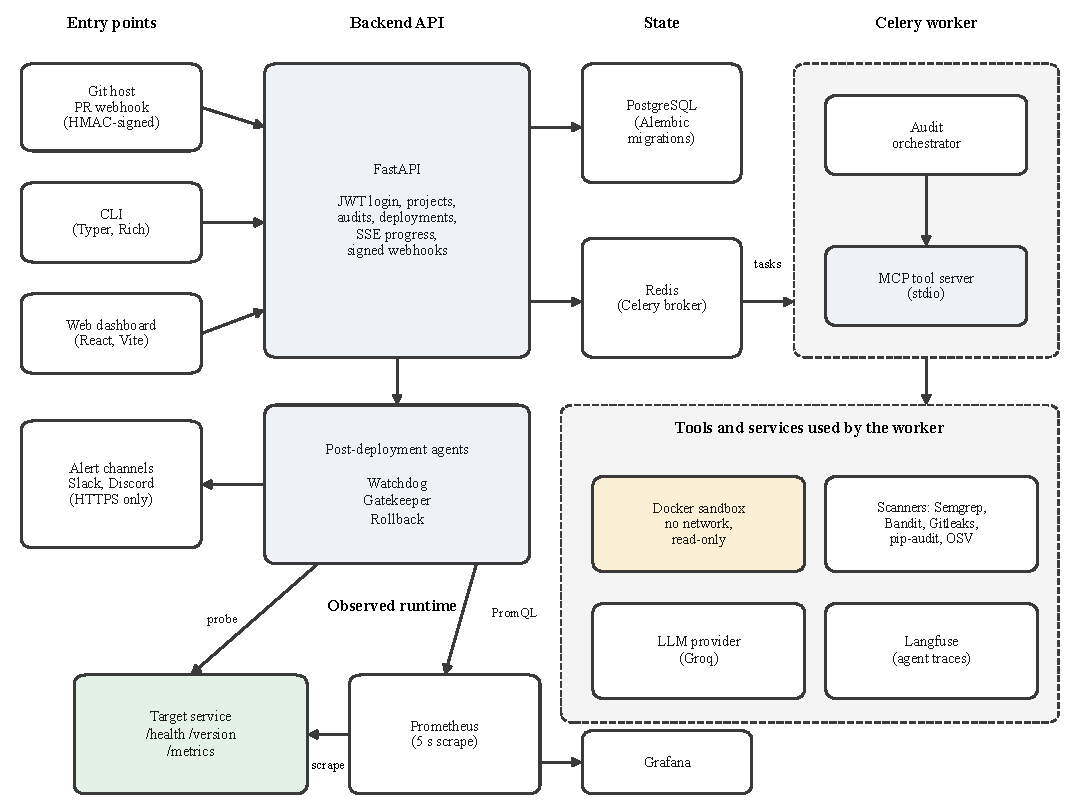
\includegraphics[width=.98\linewidth]{figures/architecture.pdf}
\caption{Sceptic architecture: entry points, control plane, worker and the tools it calls.}
\label{fig:architecture}
\end{figure}

\subsection{Pre-release audit and the gate}
Fig.~\ref{fig:workflow} shows the flow from input to verdict. Six agents run independently and write findings to a shared audit context. The Fact-Checker resolves every call against the installed environment. The Blind-Tester writes tests from the docstring only, so the tests do not depend on the code they judge, which is how a test oracle is kept independent \cite{barr2015}. The Security-Guard runs Semgrep \cite{semgrep} and Bandit \cite{bandit}, Leak-Hunter scans for committed secrets, Purana-Saman audits dependencies, and Jhooti-Docstring compares docstrings with behaviour. The synthesizer then computes
\begin{equation}
 S(c)=\max\Bigl(0,\;100-\sum_{f\in F_k}w(\mathrm{sev}(f))-\min\bigl(15,\;5\,|F_u|\bigr)\Bigr),
 \label{eq:score}
\end{equation}
and the verdict
\begin{equation}
 V(c)=\begin{cases}\text{BLOCK} & S(c)<65,\\ \text{APPROVE} & S(c)\ge 85\ \text{and}\ I(c)=0,\\ \text{REQUEST\_CHANGES} & \text{otherwise.}\end{cases}
 \label{eq:verdict}
\end{equation}
Capping the penalty for unverified checks at 15 in Eq.~\eqref{eq:score} keeps a missing tool from outweighing a real defect, while the term $I(c)$ in Eq.~\eqref{eq:verdict} ensures that code that was never audited cannot be approved. The deployment runner admits a release only on APPROVE, or on a named approver's written reason, and treats a missing verdict as unverified. Generated tests and the audited code are both untrusted, so they run in a container with no network, a read-only code mount, a small temporary filesystem, no Linux capabilities, a non-root user and limits on memory, processes and processor time \cite{dockerrun}. If Docker or the sandbox image is missing, nothing runs on the host and the agent reports a high-severity finding, so a missing sandbox can never produce an approval. Findings that quote a secret store only a short prefix of it, and the model never sees the implementation when it writes tests.
\begin{figure}[htbp]\centering
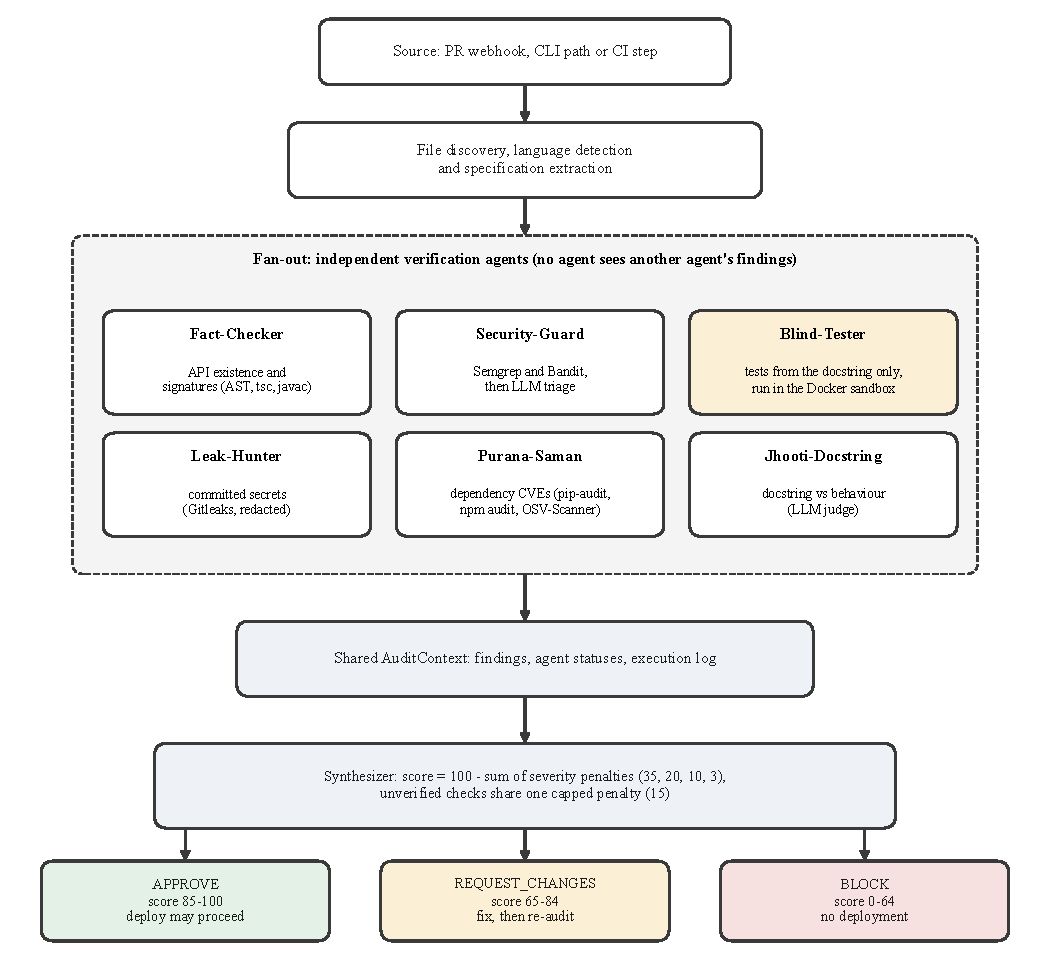
\includegraphics[width=.9\linewidth]{figures/audit_workflow.pdf}
\caption{Workflow of one audit, from input to verdict. Only the synthesizer produces a verdict.}
\label{fig:workflow}
\end{figure}

\subsection{Integration into the CI/CD pipeline}
The gate sits inside the delivery workflow as one stage. The continuous-integration workflow runs the test suites of every service, builds the frontend and all container images, and installs scanner binaries only after verifying their checksums, so the tools that do the checking are themselves pinned. The delivery workflow publishes images tagged with the commit identifier, audits the service being deployed, and passes the verdict to a deployment runner. The runner fails closed: it halts on BLOCK, on REQUEST\_CHANGES and on a missing verdict, and it accepts an override only with a named approver and a written reason of at least ten characters, which is recorded in the result. It then registers a deployment record in state DEPLOYING, polls the health and version endpoints of the target, and sets ACTIVE only if the service is healthy and reports the expected commit. A timeout or a mismatch sets FAILED and does not trigger a rollback by itself, because a person should decide whether the previous version is the right recovery.

\subsection{Runtime protection and rollback}
After release the Watchdog flags a failure when
\begin{equation}
 W(d)=\bigl[h\neq\text{healthy}\bigr]\ \lor\ \bigl[n\ge N_{\min}\ \land\ (e>\tau_e\ \lor\ \ell_{95}>\tau_\ell)\bigr],
 \label{eq:watchdog}
\end{equation}
where the minimum-sample term of Eq.~\eqref{eq:watchdog} stops a few failed requests on an idle service from raising an alarm. Missing metrics are reported as unresolved, never as a pass. A Watchdog failure and a finished rollback are sent to Slack or Discord over HTTPS, and delivery errors are logged and ignored so that alerting can never change an outcome. The Gatekeeper compares commit, version, environment and image digest with $d$ and records each distinct drift once. A rollback may run only if
\begin{equation}
 R(d)=\bigwedge_{i=1}^{5}p_i(d),
 \label{eq:rollback}
\end{equation}
where, in Eq.~\eqref{eq:rollback}, $p_1$ to $p_5$ require a valid earlier deployment in the same project, a matching environment, a well-formed image reference, a safe migration state, and no other rollback holding the project lock. Algorithm~\ref{alg:rollback} gives the procedure and Fig.~\ref{fig:deploy} shows where it sits in the release flow. Success requires the health endpoint and the running commit to match the target afterwards, and a stale lock expires so that a crashed rollback cannot block a project forever.
\begin{algorithm}[htbp]
\caption{Controlled rollback}\label{alg:rollback}
\KwIn{Deployment $d$, reason $r$, optional target $t$}
\KwOut{Record with status SUCCESS, ABORTED or FAILED}
\lIf{$r$ is empty or $d$ is already rolled back}{\Return ABORTED}
Select the target: $t$ if given, else the recorded previous deployment, else the latest earlier non-failed one\;
Evaluate $p_1,\dots,p_5$ and store the checklist\;
\lIf{$R(d)$ is false}{\Return ABORTED (service untouched)}
Take the project lock, run the configured command without a shell, wait for readiness\;
\eIf{health is healthy \textbf{and} running commit equals target commit}{set $d$ to ROLLED\_BACK and the target to ACTIVE\; \Return SUCCESS\;}{set $d$ to FAILED\; \Return FAILED with diagnostics\;}
\end{algorithm}
\begin{figure}[htbp]\centering
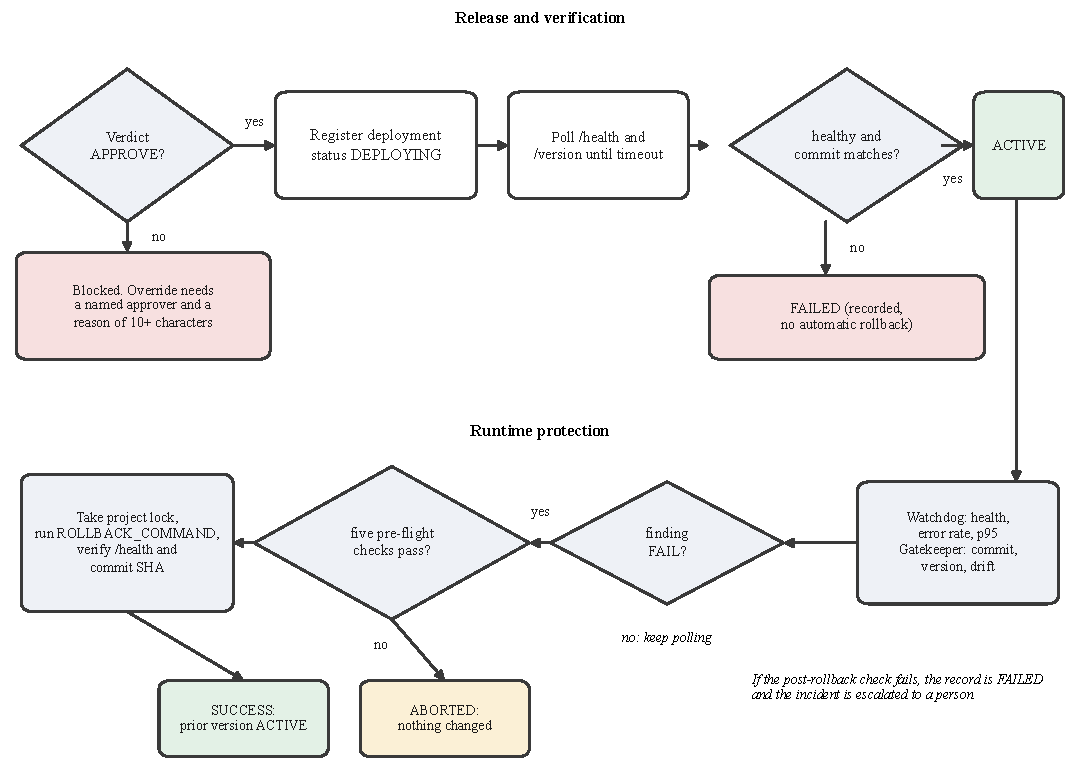
\includegraphics[width=.98\linewidth]{figures/deploy_recover.pdf}
\caption{Release verification followed by runtime protection and rollback.}
\label{fig:deploy}
\end{figure}

\subsection{Guardrails and tracing}
Docstrings, user questions and agent messages are untrusted. A two-stage guard blocks text $x$ when
\begin{equation}
 G(x)=\pi(x)\ \lor\ \bigl[s(x)\ge\tau_g\bigr],
 \label{eq:guard}
\end{equation}
where, in Eq.~\eqref{eq:guard}, $\pi$ checks length, control characters, instruction-override phrases and abusive language, and $s$ is the score of a hosted safeguard classifier \cite{promptguard}, a model of the kind introduced by Llama Guard \cite{inan2023}. A blocked docstring does not stop the audit: the agent records an unresolved finding and does not call the model. Patterns are cheap but brittle, and a classifier generalises better but costs time, so the guard uses both. Every audit produces one Langfuse trace with a span per agent, tool call and model call, and by default spans carry sizes and hashes, not source text. The trace identifier is stored with the audit and linked from the dashboard, so a reviewer can see which agent produced each finding. Automatic rollback after a Watchdog failure is off by default, because the Watchdog probes one shared target and its failure does not identify a deployment.

\section{Experimental Setup}
\textbf{Data.} The benchmark has 27 Python files written by the authors and labelled in a manifest: 12 seeded defects (4 non-existent standard-library calls, 3 specification mismatches such as an addition function that multiplies, and 5 security defects) and 15 clean files that use similar libraries. No training or split is involved. The guardrail sets are labelled text: a tuning set (25 attacks, 25 benign) used to develop the pattern rules and a held-out set (15 attacks, 20 benign) written afterwards.

\textbf{Environment.} Experiments ran on a Windows 11 laptop with Python 3.12.3, Semgrep 1.179.0, Bandit 1.9.4, CrewAI 1.15.23, google-adk 2.13.0, MCP 1.29.0 and Docker engine 29.8.2. The language model was \texttt{openai/gpt-oss-120b} served by Groq, and the classifier was Llama Prompt Guard 2 (86M).

\textbf{Baselines.} \emph{Build only} byte-compiles each file, which is what a build gate checks. \emph{Bandit only} runs one security scanner, as many pipelines do, and counts findings of medium or high severity. Both are deterministic, so their spread over repeats is zero.

\textbf{Metrics.} The \emph{catch rate} is the share of seeded defects detected, since this is the value of a gate. A defect is caught only when an agent responsible for its category reports a finding of medium severity or higher: the Fact-Checker for non-existent APIs, the Security-Guard or Leak-Hunter for security defects, and the Blind-Tester for specification mismatches, where the finding must also be an assertion failure from a generated test. This stricter rule stops an agent that fires on every file from being credited with detections it is not responsible for. The \emph{false-positive rate} is the share of clean files that receive a finding of medium severity or higher from any agent, because false alarms make teams bypass gates \cite{johnson2013}. We also report seconds, tokens and dollars per audit, because they set the delay and budget of a pipeline, and for the guardrail the share of attacks and of benign inputs blocked.

\textbf{Parameters.} Table~\ref{tab:params} lists every setting. Each configuration was run three times over all 27 files. No random seed was fixed, because the model is sampled by the provider.
\begin{table}[htbp]\centering
\caption{Parameters and settings used in all experiments.}
\label{tab:params}\small
\begin{tabular}{@{}p{.34\linewidth}p{.58\linewidth}@{}}\toprule
Setting & Value\\\midrule
Repeats, files per repeat & 3 repeats, 27 files, in each of the two modes\\
Modes & With language model; without (provider key empty)\\
Random seed & Not fixed (model sampled by the provider)\\
Pacing between audits & 15 s (model mode), to stay under 8,000 tokens per minute\\
Penalties $w$, uncertainty cap & 35, 20, 10, 3, 0; cap 15\\
Verdict thresholds & APPROVE $\ge 85$, BLOCK $<65$\\
Sandbox limits & No network, read-only mount, 128 MB temp, 512 MB memory, 1 CPU, 256 processes, user 65534, no capabilities\\
Watchdog & $N_{\min}=10$, $\tau_e=5\%$, $\tau_\ell=0.5$ s, 5-minute window\\
Guardrail & Pattern stage, then classifier with $\tau_g=0.5$\\
Price assumed & \$0.15 and \$0.60 per million input and output tokens (third-party listings)\\
\bottomrule\end{tabular}
\end{table}

\section{Results and Analysis}
\subsection{RQ1: Detection against the baselines}
Table~\ref{tab:main} compares the configurations over three repeats of all 27 files. The build-only pipeline caught none of the 12 seeded defects, which is expected, because every seeded file is valid Python. Bandit alone caught 4 of 12 (33.3\%), all of them security defects, and flagged no clean file. The full agent set without a language model caught 9 of 12 (75.0\%) in every repeat, so its standard deviation is zero. These figures come from the same 81 audits used for the ablation below.
\begin{table}[htbp]\centering
\caption{Seeded defects caught and clean files flagged per configuration, as mean $\pm$ sample SD over three repeats. The best catch rate is in bold.}
\label{tab:main}\small
\begin{tabular}{@{}p{.40\linewidth}rrr@{}}\toprule
Configuration & Caught (\%) & Flagged (\%) & Seconds per audit\\\midrule
Build only (baseline) & 0.0 $\pm$ 0.0 & 0.0 $\pm$ 0.0 & ---\\
Bandit only (baseline) & 33.3 $\pm$ 0.0 & 0.0 $\pm$ 0.0 & ---\\
Sceptic, no language model & 75.0 $\pm$ 0.0 & 93.3 $\pm$ 0.0 & 6.17 $\pm$ 0.23\\
Sceptic, all six agents, with model & \textbf{83.3} $\pm$ 0.0 & 48.9 $\pm$ 7.7 & 10.72 $\pm$ 1.34\\
\bottomrule\end{tabular}
\end{table}
With the language model on, the full agent set caught 10 of 12 seeded defects (83.3\%) in every repeat and flagged 48.9\% of the clean files, which is 6, 8 and 8 of 15 in the three repeats (last row of Table~\ref{tab:main}).
The categories show where the baselines fall short. All four non-existent API calls were caught by the Fact-Checker, which no baseline can do because it requires resolving names against the installed environment. All five security defects were caught, four by the Security-Guard and the hard-coded password by Leak-Hunter. None of the three specification mismatches was caught without a model, because the fallback tests do not contradict a wrong implementation. With the model, the Blind-Tester caught the function that returns the smaller of two numbers and missed the addition that multiplies and the floor division in all three repeats, which is the one extra detection in the last row. Fig.~\ref{fig:results}(a) shows the catch rates and Fig.~\ref{fig:results}(b) the false-positive rates side by side.
\begin{figure}[htbp]\centering
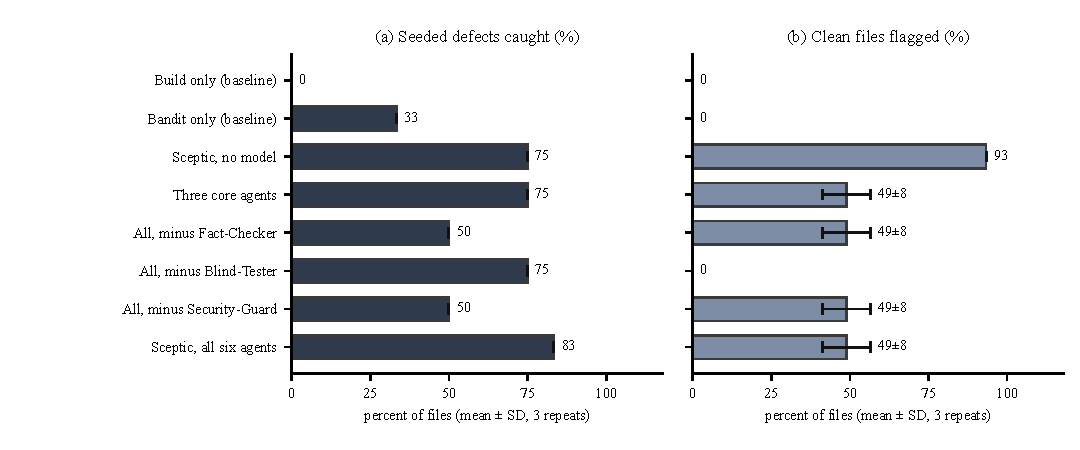
\includegraphics[width=.98\linewidth]{figures/results.pdf}
\caption{(a) Seeded defects caught and (b) clean files flagged, by configuration. Bars show the mean and error bars the sample standard deviation over three repeats.}
\label{fig:results}
\end{figure}

The false-positive column looks much worse. Without a model, 14 of 15 clean files (93.3\%) were flagged in every repeat, and every flagged finding was a failed fallback test of the Blind-Tester. Bandit flagged none of the clean files, and it also missed eight of the twelve defects. With the model the rate falls to 48.9\% (6 to 8 of 15 files), and again every flagged finding came from the Blind-Tester, in 12 different clean files. Fig.~\ref{fig:results}(b) shows the cost of the extra detections: a false-positive rate this high would make the gate unusable as a blocking stage.
\subsection{RQ2: Ablation, cost and guardrail}
Table~\ref{tab:ablation} removes one agent at a time from the model-mode runs, using the same audits as Table~\ref{tab:main}. The drop in catch rate when an agent is removed measures what that agent contributes, and the drop in flagged files measures the false alarms it causes. Removing the Fact-Checker or the Security-Guard cuts the catch rate from 83.3\% to 50.0\%, because each is the only agent that catches its four defects, and neither changes the false-positive rate. Removing the Blind-Tester costs one detection (75.0\%) but takes the false-positive rate from 48.9\% to 0.0\%, so that single agent produces all of the false alarms. The three core agents reach 75.0\% against 83.3\% for all six, and the difference is the hard-coded password, which only Leak-Hunter reports at a usable severity.
\begin{table}[htbp]\centering
\caption{Ablation: configurations with one agent removed, over three repeats (mean $\pm$ SD).}
\label{tab:ablation}\small
\begin{tabular}{@{}p{.40\linewidth}rr@{}}\toprule
Configuration & Caught (\%) & Flagged (\%)\\\midrule
All six agents & \textbf{83.3} $\pm$ 0.0 & 48.9 $\pm$ 7.7\\
Without Fact-Checker & 50.0 $\pm$ 0.0 & 48.9 $\pm$ 7.7\\
Without Blind-Tester & 75.0 $\pm$ 0.0 & \textbf{0.0} $\pm$ 0.0\\
Without Security-Guard & 50.0 $\pm$ 0.0 & 48.9 $\pm$ 7.7\\
Three core agents only & 75.0 $\pm$ 0.0 & 48.9 $\pm$ 7.7\\
\bottomrule\end{tabular}
\end{table}

Cost is shown in Fig.~\ref{fig:cost}(a). With the sandbox running and no model, an audit took 6.17 $\pm$ 0.23 s on average over three repeats, most of it spent in the Security-Guard's scanners. With the model, the average audit took 10.72 $\pm$ 1.34 s, about 4.5 s longer, because it made 2.89 model calls and used 585.5 input and 1,134.0 output tokens. At the assumed price that is about \$0.00077 per audit, or \$0.77 per thousand audits. No model call failed in any of the 81 audits. The model run was paced at 15 s between audits to stay under the provider's tokens-per-minute limit, and the pause is not counted in the audit time.

The guardrail is a separate ablation, since it protects the agent layer and not the gate's verdict. Table~\ref{tab:guard} shows that on the tuning set the pattern stage blocked all 25 attacks without blocking a benign input, which only shows that the rules fit the examples they were written from. On the held-out set it blocked 5 of 15 attacks (33\%) and wrongly blocked 2 of 20 benign inputs (10\%). Adding the classifier raised the blocked attacks to 13 of 15 (87\%) and left the two false blocks unchanged. Both false blocks were ordinary documentation that contained a trigger term, the phrase ``developer mode'' and the string ``kys'' used as a configuration key. The classifier's gain costs time: patterns take 0.02 ms per input and the classifier 1.4 to 2.7 s, partly from retries after rate-limit responses, so scores are cached by text. Two attacks passed both stages, so the guardrail lowers the risk without removing it.
\begin{table}[htbp]\centering
\caption{Input guardrail ablation: patterns only against patterns plus classifier.}
\label{tab:guard}\small
\begin{tabular}{@{}p{.17\linewidth}p{.24\linewidth}p{.15\linewidth}p{.15\linewidth}p{.13\linewidth}@{}}\toprule
Set & Stages & Attacks blocked & Benign blocked & Time per input\\\midrule
Tuning (25 + 25) & Patterns & 25/25 & 0/25 & 0.02 ms\\
Tuning (25 + 25) & Patterns + classifier & 25/25 & 2/25 & 1.4 s\\
Held-out (15 + 20) & Patterns & 5/15 & 2/20 & 0.02 ms\\
Held-out (15 + 20) & Patterns + classifier & \textbf{13/15} & 2/20 & 2.7 s\\
\bottomrule\end{tabular}
\end{table}
\begin{figure}[htbp]\centering
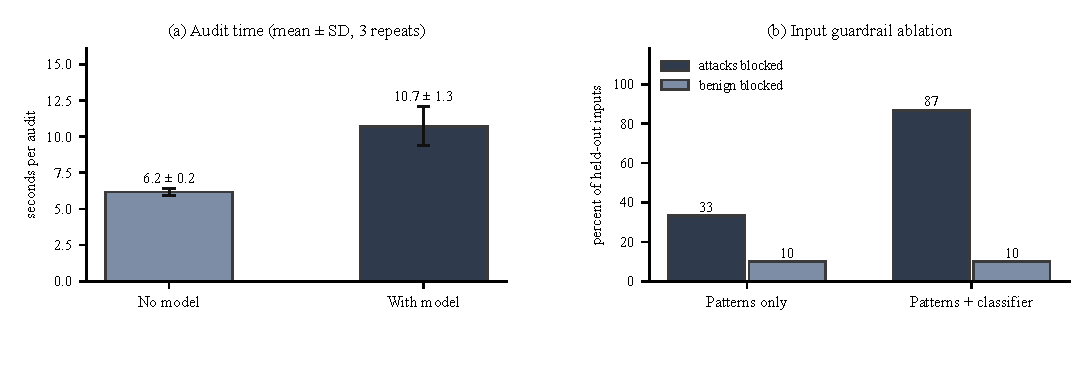
\includegraphics[width=.98\linewidth]{figures/cost.pdf}
\caption{(a) Audit time with and without the language model (mean $\pm$ SD over three repeats). (b) Attacks and benign inputs blocked on the held-out guardrail set.}
\label{fig:cost}
\end{figure}

\section{Discussion}
A build gate is not enough for generated code. Byte-compiling caught nothing, because every seeded file is valid Python, and Bandit alone caught a third of the defects, all of them security patterns. Neither can see a fabricated call or a function that contradicts its docstring, which are the errors assistants add \cite{spracklen2025}. The signature check closes the first gap deterministically. The hard-coded password was caught because Leak-Hunter reports it, whereas Bandit reports the same string only at low severity.

That coverage comes with the Blind-Tester's false positives. Without a model, 14 of 15 clean files were flagged, and with the model 6 to 8, and in both cases every flagged finding was a failed test of that agent. We did not investigate the cause further, so we can only say that its generated and fallback assertions are not a reliable oracle for correct code \cite{barr2015}. The agent earns one of the ten detections, the specification mismatch that no other agent can see. A gate that blocks nearly every change will be bypassed \cite{johnson2013}, so until the Blind-Tester is repaired it should run in an advisory role, and the blocking verdict should come from the other agents, whose false-positive rate in our runs was zero.

\textbf{Limitations.} The benchmark is small, was written by the authors, covers Python only and uses single-function files, so the catch rates carry wide uncertainty and say little about real repositories. The zero spread over repeats of the no-model configuration comes from deterministic components and says nothing about robustness. The post-release agents were verified by automated tests and not by live fault runs. Injecting faults deliberately, as chaos engineering does \cite{basiri2016}, is the natural next measurement. The cost figure uses a third-party price. The guardrail held-out set was scored once and a rule was changed afterwards, so it can no longer serve as a clean test.

\textbf{Threats to validity.} Our scripts decide what counts as caught, and a different rule would shift the numbers. The model is sampled by the provider with no fixed seed, so three repeats cannot show every source of variation. A scoring or implementation error is possible, which is why the raw findings of every run are stored and each reported number can be recomputed.

\textbf{Ethics.} Sending source code to a hosted model discloses it to a third party, so tracing exports only sizes and hashes by default. An automatic rollback can interrupt a working service, so it is off by default. The text of this paper was drafted with an AI model and is declared as such.

\section{Conclusion and Future Work}
RQ1: the agent gate caught 75.0\% of the seeded defects without a language model and 83.3\% with one, against 0\% for a build-only pipeline and 33.3\% for Bandit alone, but it flagged 93.3\% of the clean files without a model and 48.9\% with one. RQ2: the Fact-Checker and the Security-Guard each contribute four of the ten detections, and the Blind-Tester contributes one detection and all of the false alarms. An audit took 6.2 s without a model and 10.7 s with one, at about \$0.77 per thousand audits, and the classifier raised the share of unseen attacks blocked from 33\% to 87\% at a cost of 1.4 to 2.7 s per input.

The main result is a trade-off. The gate detects fabricated calls and committed secrets, which a build and a single scanner miss, but the Blind-Tester makes it too noisy to run as a blocking stage until its tests are fixed. We see three next steps. First, repair the Blind-Tester, for example by validating generated tests against known-correct code before trusting them, and re-measure the false-positive rate on the 15 clean files. Second, run the full stack with deliberate fault injection and report time to detect and time to restore, which this paper could not measure. Third, enlarge the benchmark beyond single-function Python files, add other languages, and deploy the platform with HTTPS, a production frontend image and per-deployment probe targets.

\noindent\textbf{Git repository:} \url{https://github.com/[owner]/[repository]}.

\section*{AI-use declaration}
An AI model (Claude, from Anthropic, used through Claude Code) helped read the repository, run the evaluation scripts, draw the figures and draft this manuscript. [The authors must replace this paragraph with an accurate account of which parts they wrote themselves, how they checked every number against evaluation/results/, and how they read every cited source.]

\section*{Member contributions}
\noindent\textbf{Suvansh Sehgal}: [One verified sentence about his contribution.]\\
\textbf{Anubhav Jhanwar}: [One verified sentence about his contribution.]\\
\textbf{Dev Garg}: [One verified sentence about his contribution.]

\bibliographystyle{IEEEtran}
\bibliography{references}
\end{document}
